%
% File: chap02.tex
%
\let\textcircled=\pgftextcircled
\chapter{Experimental Results}
\label{Chapter4}

\section{Technical details and implementation}
playing with the parameters
\subsection{Feature generation}
\cite{deepwalk_hyper} carried out a research for community detection using DeepWalk. After some experiments, they found convienent that for its problem the following parameters were eno 
As specified by Perozzi et. al.~\cite{deepwalk}, their experiments suggest that the number of walks started per vertex should be greater or equal than $\gamma=30$, the latent dimension greater or equal than $d=64$, and they fixed the sensible values of $w=10$ for the window size, and $t=40$ for the walk length . Based on those recommendations, in the experiments carried out in~\cite{deepwalk_hyper}, and the computational needs of the problem to be solved, it was found convenient to set $\gamma=60$, $d=64$, $w=15$, and $t=80$.

Taking into account the computational needs of the problem to be solved, and some 

Saving and manipulating only the adjacency lists instead of the whole adjacency matrix, is an important 

For the algorithm that is proposed here, the implementation by the Karate Club API~\cite{karateclub} was used.
The number of partitions was set to four differently from the original paper where three partitions were used. It was used this number of partitions to have a comparison point with the result in The Graph Partitioning archive. There, the number of partitions is always a power of $2$.

Quality metrics

METIS was used from the networkx interface

\section{Dataset}

    For the dataset used to train and test the algorithm "The Graph Partitioning Archive"~\cite{archive}
The graphs are in the standard format used by JOSTLE and METIS. A description of the format and the requirements can be found in~\cite{jostle}.

For the purposes of this research, the graphs contained in "The Graph Partitioning Archive" where categorized in one of the following categories according to their vertex cardinality: 
\begin{itemize}
    \item Tiny graphs: those with less than $10,000$ nodes,
    \item Small graphs: those with node size between $45,000$ and $75,000$ and,
    \item Medium graphs: those with at least $99,000$ nodes but no more than $500,000$.
\end{itemize}

Ask Luis: is there a word for graphs with size more than big

\begin{table}[h!]
\centering
\begin{tabular}{ |p{1.75cm}||cc|  }
\hline
\multicolumn{3}{|c|}{\textbf{Computation Graphs}} \\
\hline
\hline
\textbf{Name} & \textbf{Nodes} & \textbf{Edges} \\
\hline
data & 2851 & 15093  \\
add32 & 4960 & 9462  \\
bcsstk33 & 8738 & 291583  \\
crack & 10240 & 30380  \\
\hline
fe\_body & 45087 & 163734  \\
t60k & 60005 & 89440  \\
wing & 62032 & 121544  \\
finan512 & 74752 & 261120 \\
\hline
fe\_rotor & 99617 & 662431  \\
598a & 110971 & 741934  \\
m14b & 214765 & 1679018	 \\
auto & 448695 & 3314611  \\
\hline
\end{tabular}
\caption{\label{tab:characteristics}Summary of the graphs characteristics. Taken from "The Graph Partitioning Archive" ~\cite{archive}}
\end{table}

%%%%%%%%%%%%%%%%%%%%%%%%%%%%%%%%%%%%%%%%%%%%%% Graph images %%%%%%%%%%%%%%%%%%%%%%%%%%%%%%%%%%%%%%%%%%%%%%%%%%%

\begin{comment}
\begin{figure}[h!]
\centering
\begin{subfigure}{.35\textwidth}
  \centering
  % include first image
  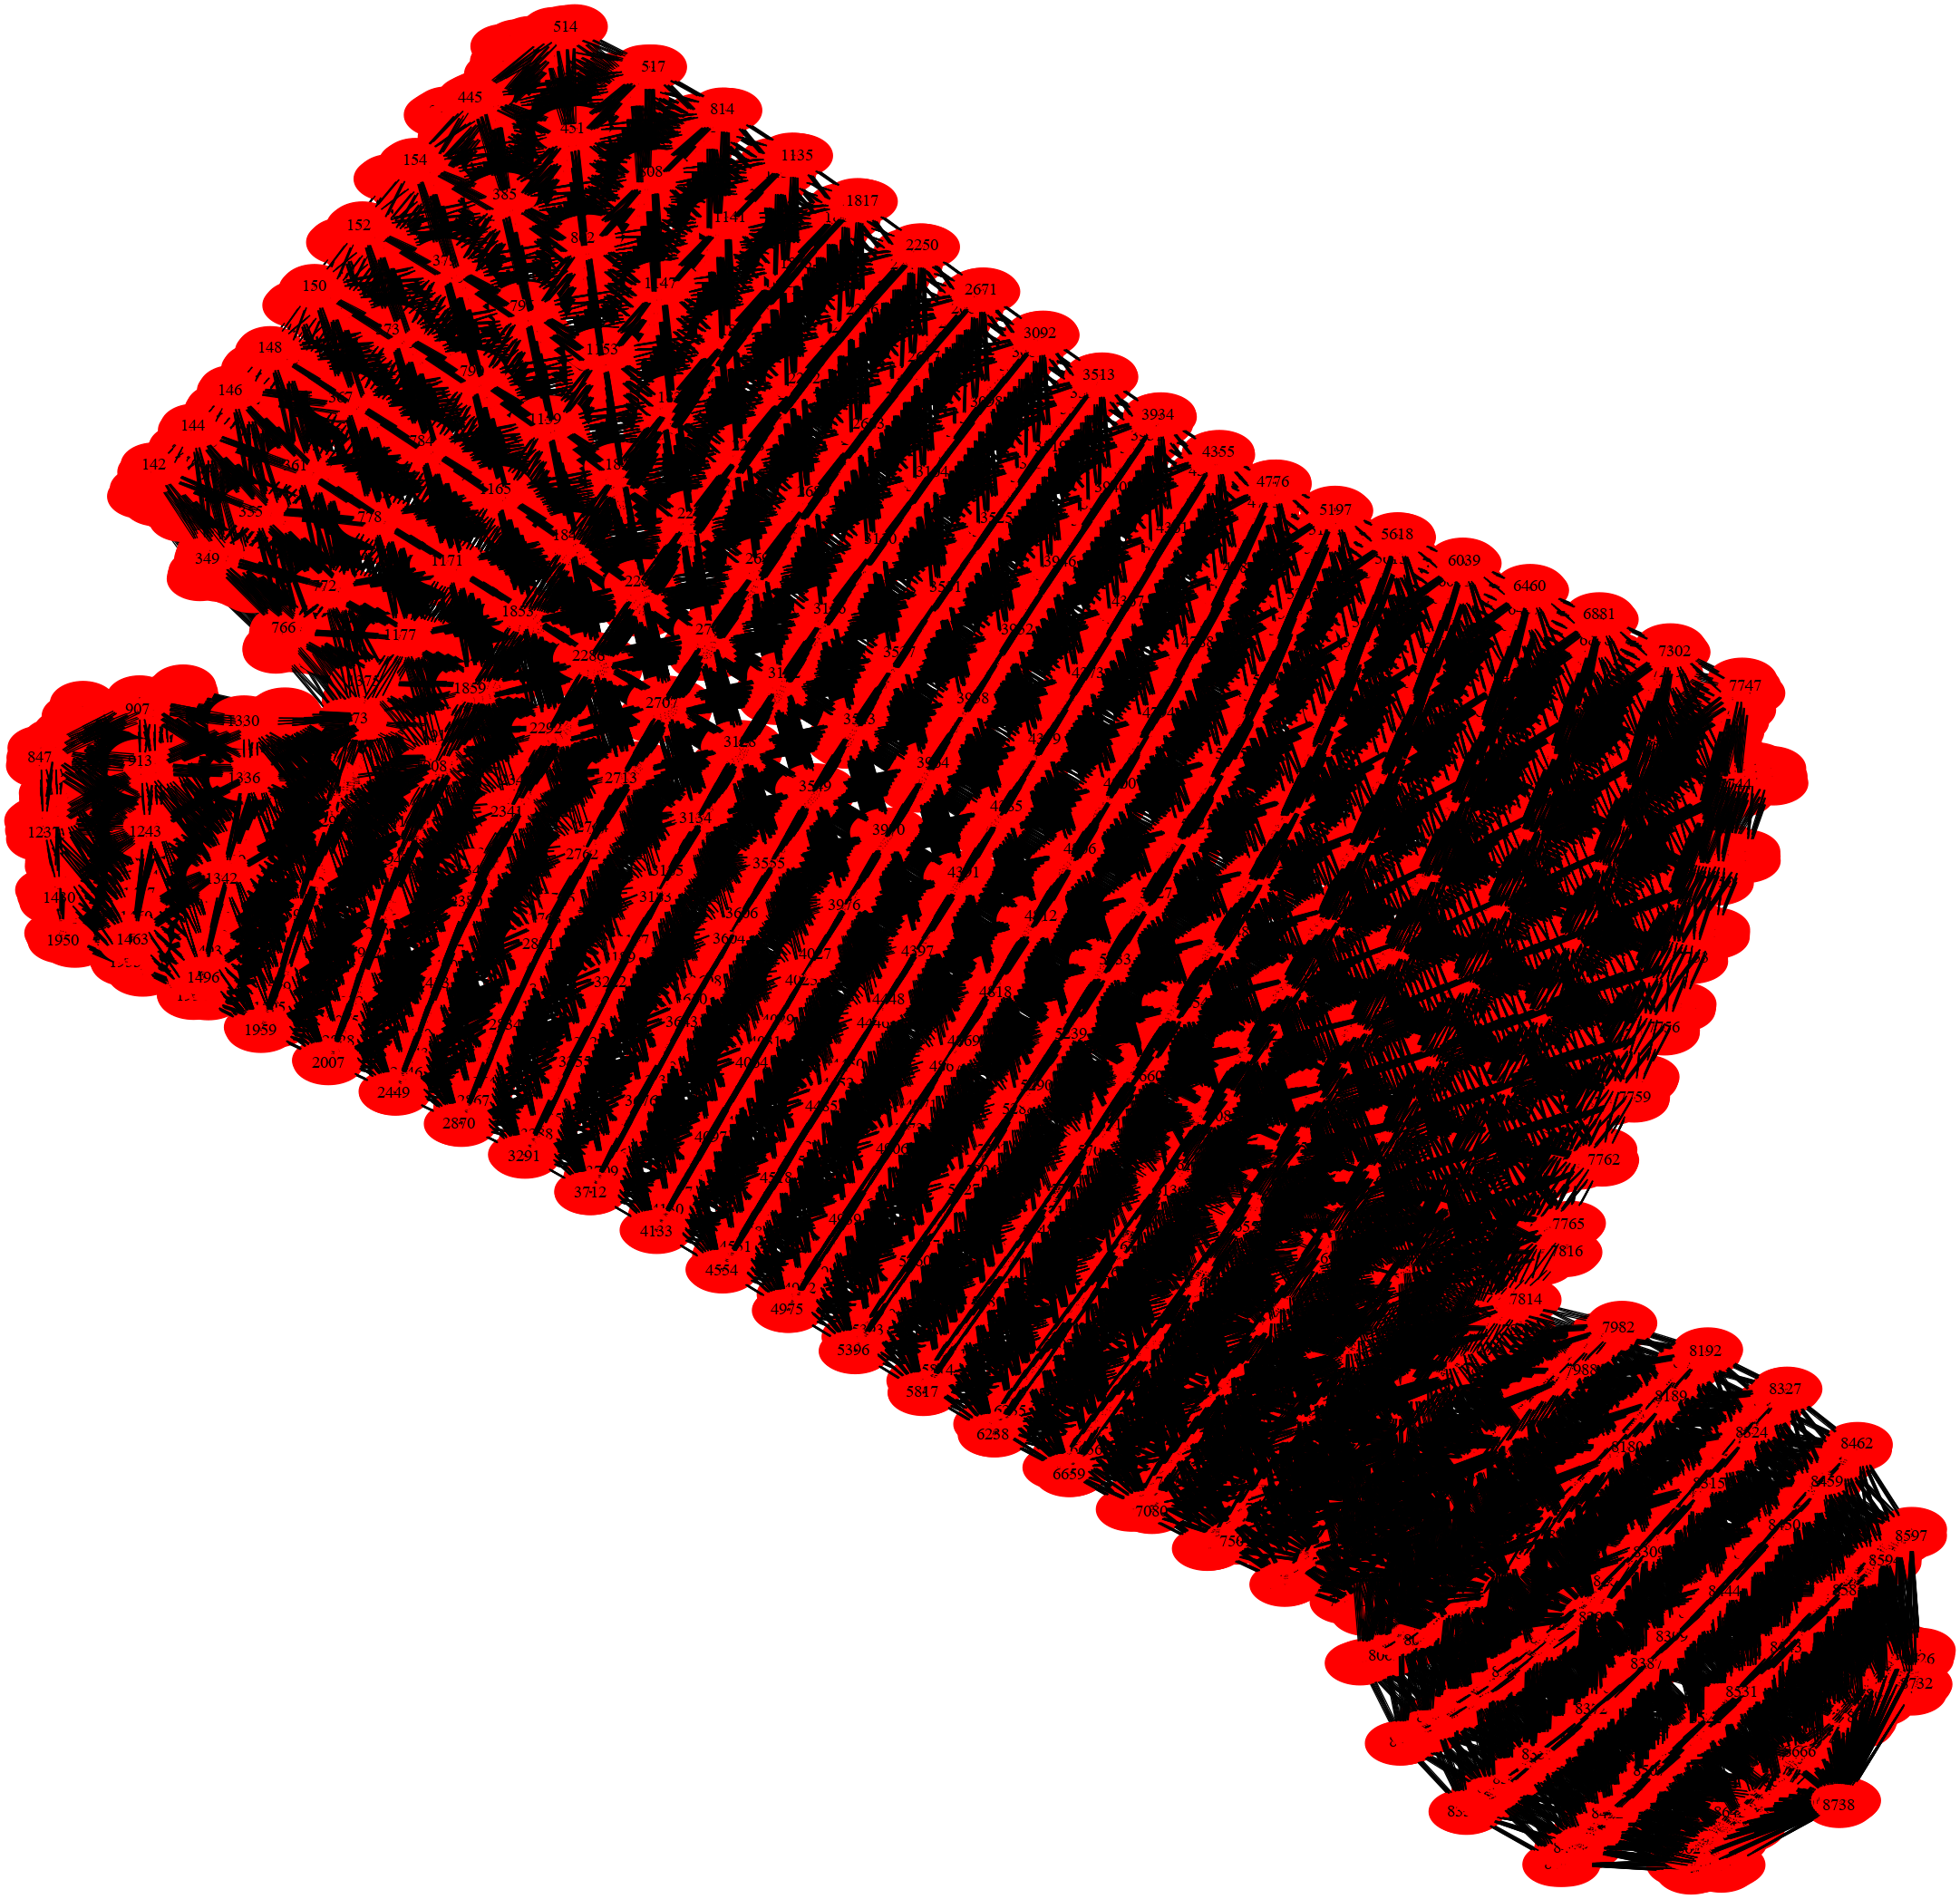
\includegraphics[width=0.7\linewidth]{graphs/bcsstk33.png}  
  \caption{bcsstk33}
  \label{fig:sub-first}
\end{subfigure}
\begin{subfigure}{.35\textwidth}
  \centering
  % include second image
  \includegraphics[width=0.7\linewidth]{graphs/crack-min.png}  
  \caption{crack}
  \label{fig:sub-second}
\end{subfigure}

\begin{subfigure}{.35\textwidth}
  \centering
  % include third image
  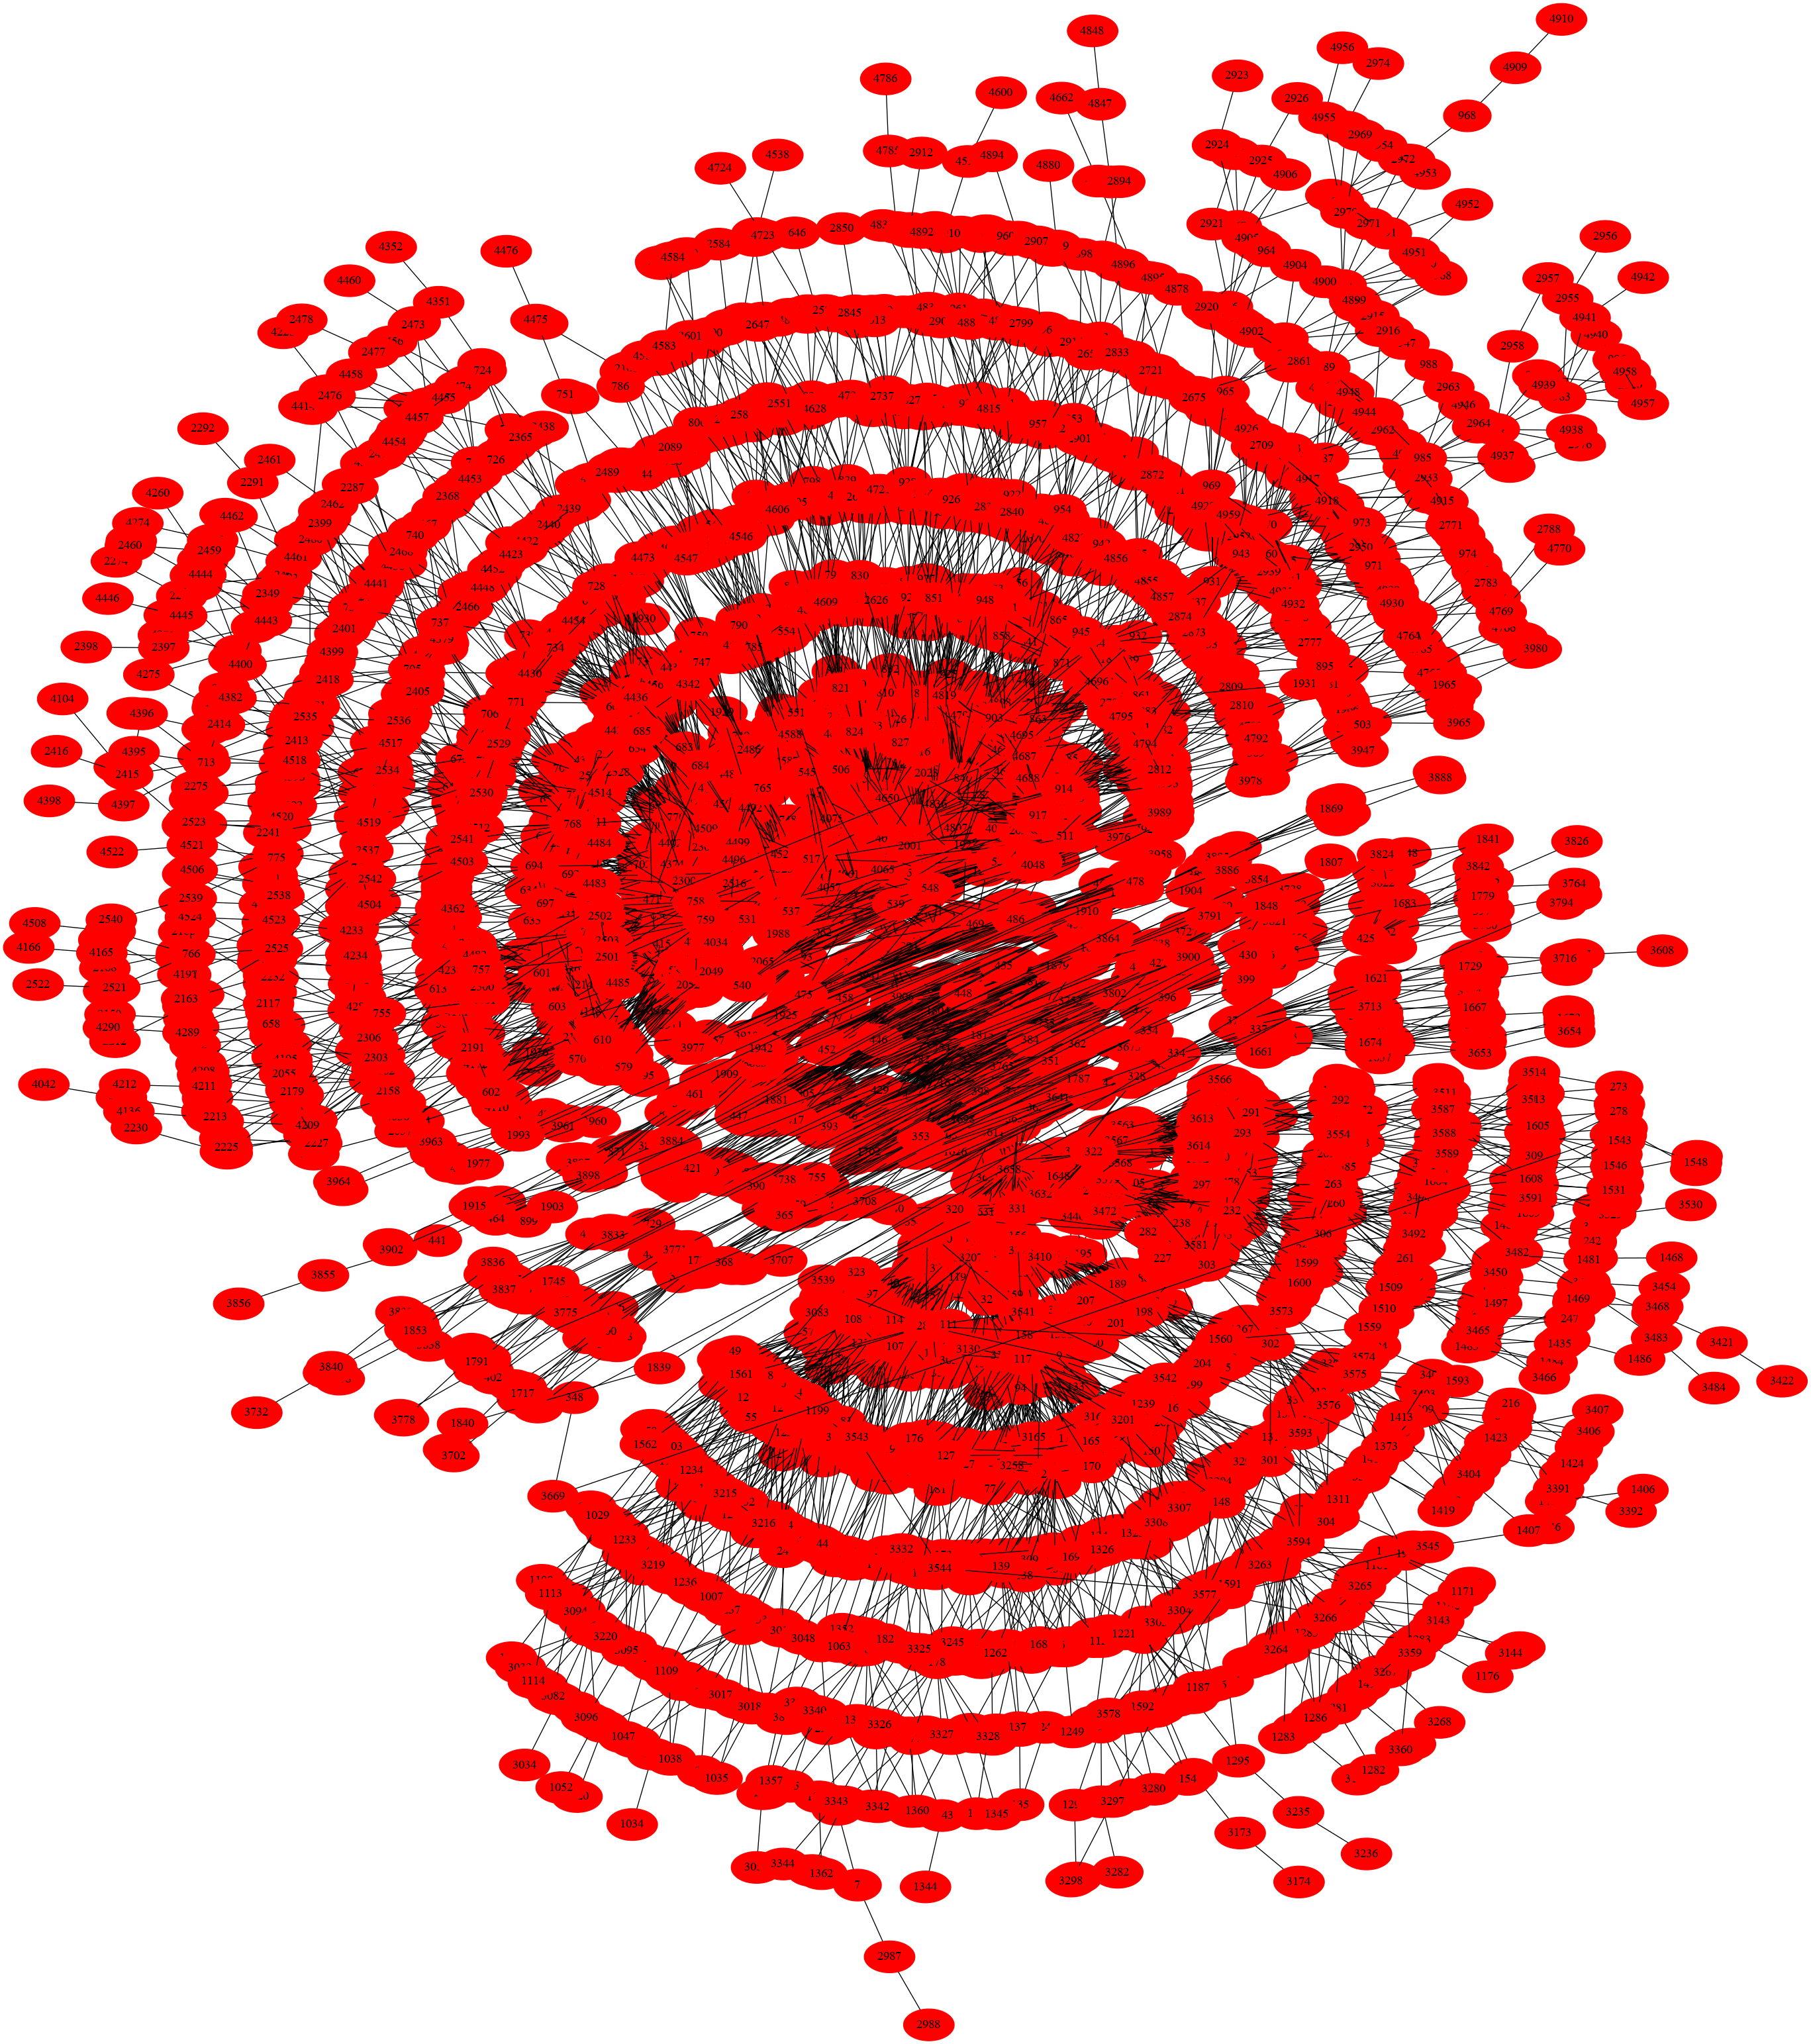
\includegraphics[width=0.7\linewidth]{graphs/add32.png}  
  \caption{add32}
  \label{fig:sub-third}
\end{subfigure}
\begin{subfigure}{.35\textwidth}
  \centering
  % include fourth image
  \includegraphics[width=0.7\linewidth]{graphs/data.png}  
  \caption{data}
  \label{fig:sub-fourth}
\end{subfigure}
\caption{Visualization of some of the graphs used in the experiments.}
\label{fig:fig}
\end{figure}
\end{comment}

%%%%%%%%%%%%%%%%%%%%%%%%%%%%%%%%%%%%%%%%%%%%%% Small graph histograms %%%%%%%%%%%%%%%%%%%%%%%%%%%%%%%%%%%%%%%%%%%%%%

\begin{figure}[h!]
\centering
\begin{subfigure}[b]{.35\textwidth}
  \centering
  % include first image
  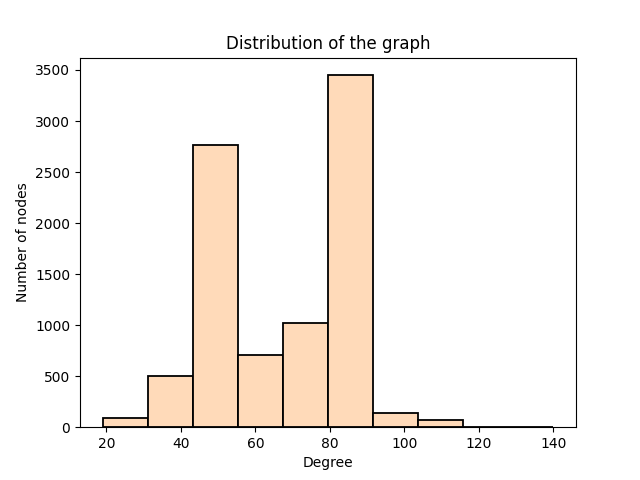
\includegraphics[width=\linewidth]{small_graphs/bcsstk33.png}  
  \caption{bcsstk33}
  \label{fig:sub-first}
\end{subfigure}
\begin{subfigure}[b]{.35\textwidth}
  \centering
  % include second image
  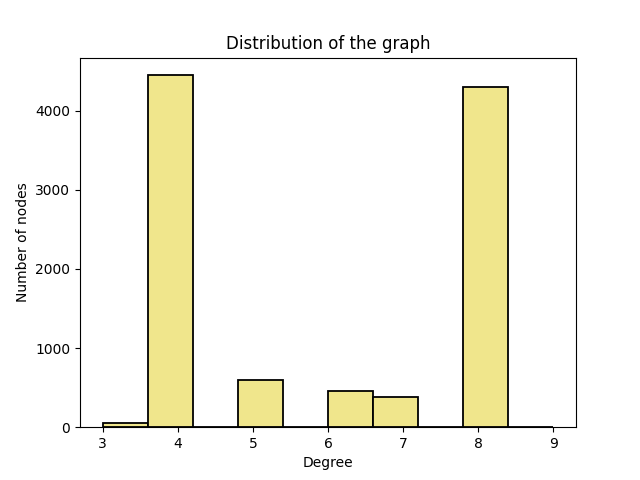
\includegraphics[width=\linewidth]{small_graphs/crack.png}  
  \caption{crack}
  \label{fig:sub-second}
\end{subfigure}

\begin{subfigure}[b]{.35\textwidth}
  \centering
  % include third image
  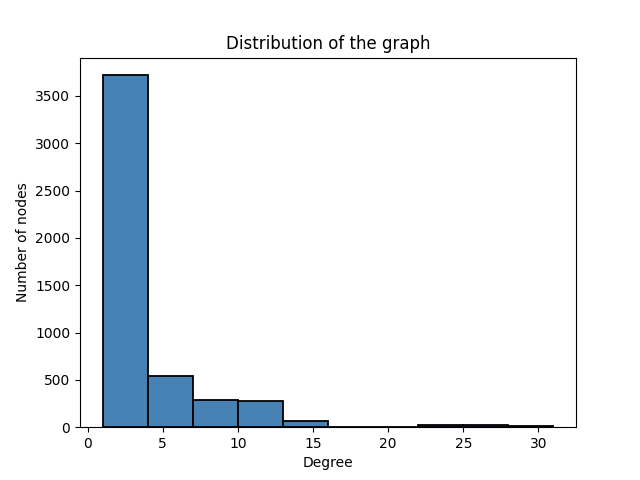
\includegraphics[width=\linewidth]{small_graphs/add32.png}  
  \caption{add32}
  \label{fig:sub-third}
\end{subfigure}
\begin{subfigure}[b]{.35\textwidth}
  \centering
  % include fourth image
  \includegraphics[width=\linewidth]{small_graphs/data.png}  
  \caption{data}
  \label{fig:sub-fourth}
\end{subfigure}
\caption{Degree histogram of small graphs: bcsstk33, crack, add32, and data. Graphs are not so dense.}
\label{fig:fig}
\end{figure}

%%%%%%%%%%%%%%%%%%%%%%%%%%%%%%%%%%%%%%%%%% Medium graph histograms %%%%%%%%%%%%%%%%%%%%%%%%%%%%%%%%%%%%%%%%%%%%%%

\begin{figure}[h!]
\centering
\begin{subfigure}{.35\textwidth}
  \centering
  % include first image
  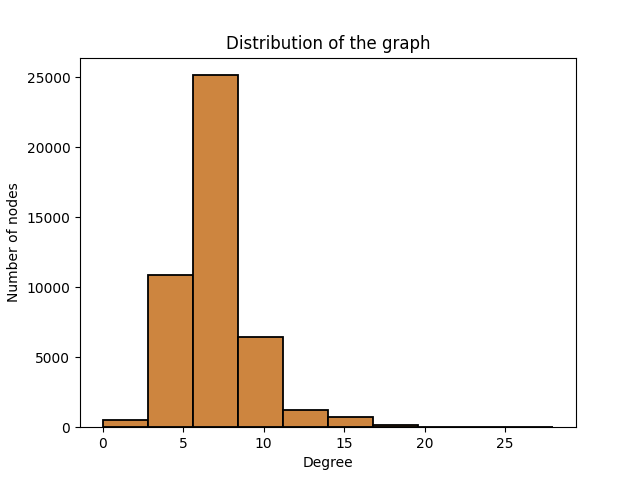
\includegraphics[width=\linewidth]{medium_graphs/fe_body.png}  
  \caption{fe\_body}
  \label{fig:sub-first}
\end{subfigure}
\begin{subfigure}{.35\textwidth}
  \centering
  % include second image
  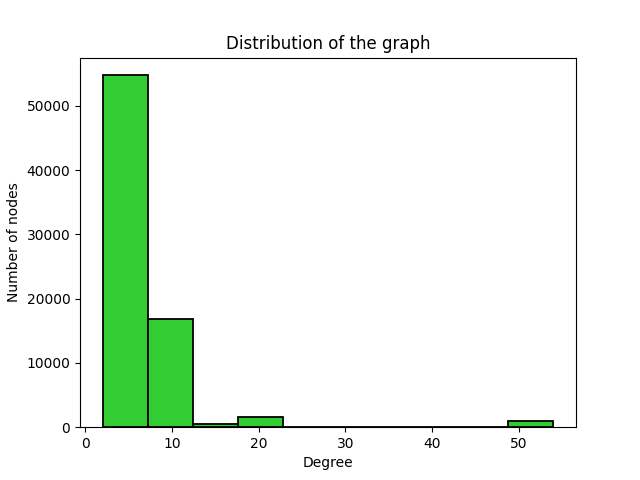
\includegraphics[width=\linewidth]{medium_graphs/finan512.png}  
  \caption{finan512}
  \label{fig:sub-second}
\end{subfigure}

\begin{subfigure}{.35\textwidth}
  \centering
  % include third image
  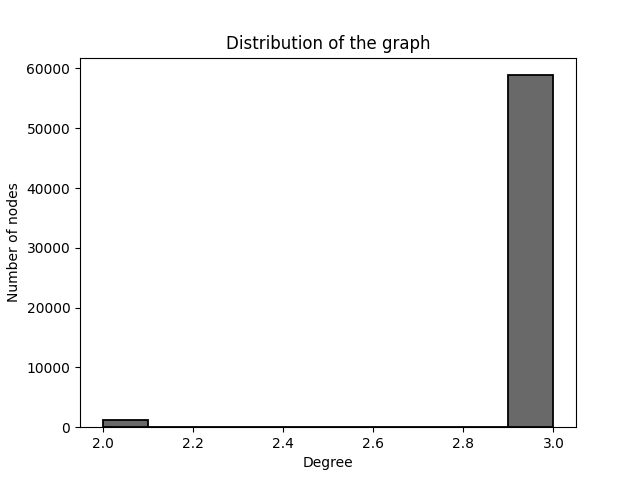
\includegraphics[width=\linewidth]{medium_graphs/t60k.png}  
  \caption{t60k}
  \label{fig:sub-third}
\end{subfigure}
\begin{subfigure}{.35\textwidth}
  \centering
  % include fourth image
  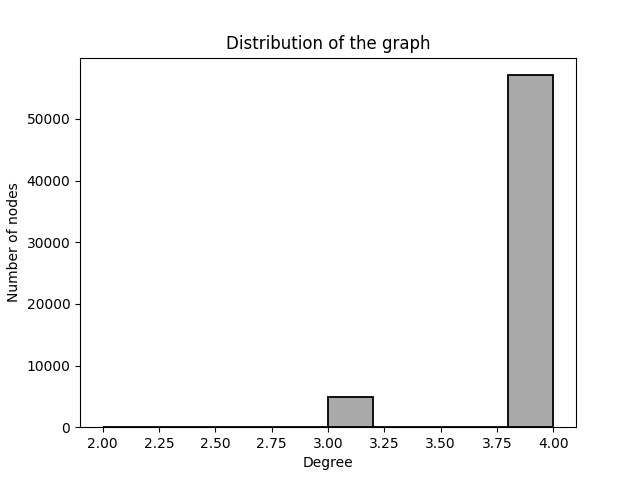
\includegraphics[width=\linewidth]{medium_graphs/wing.png}  
  \caption{wing}
  \label{fig:sub-fourth}
\end{subfigure}
\caption{Degree histogram of medium graphs. Graphs are not so dense.}
\label{fig:fig}
\end{figure}

%%%%%%%%%%%%%%%%%%%%%%%%%%%%%%%%%%%%%%%%%%%%%% Large graph histograms %%%%%%%%%%%%%%%%%%%%%%%%%%%%%%%%%%%%%%%%%%%%%%

\begin{figure}[h!]
\centering
\begin{subfigure}{.35\textwidth}
  \centering
  % include first image
  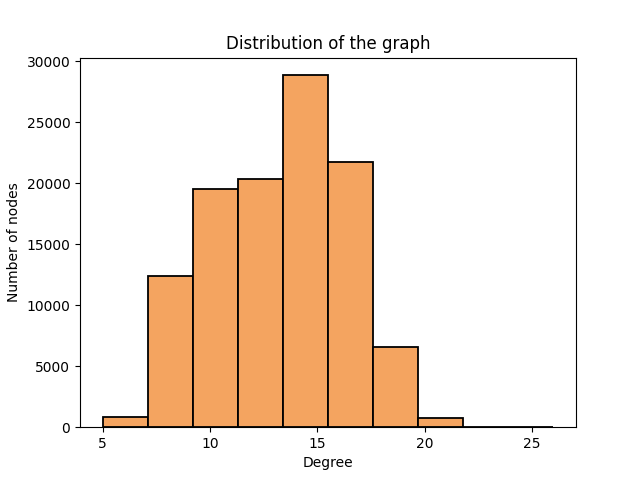
\includegraphics[width=\linewidth]{large_graphs/598a.png}  
  \caption{598a}
  \label{fig:sub-first}
\end{subfigure}
\begin{subfigure}{.35\textwidth}
  \centering
  % include second image
  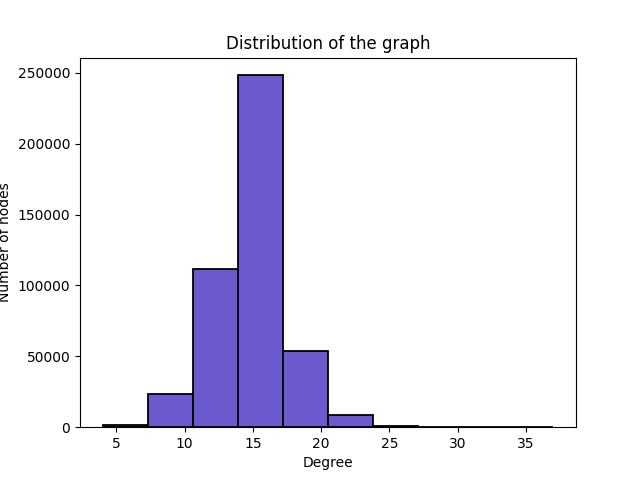
\includegraphics[width=\linewidth]{large_graphs/auto.png}  
  \caption{auto}
  \label{fig:sub-second}
\end{subfigure}

\begin{subfigure}{.35\textwidth}
  \centering
  % include third image
  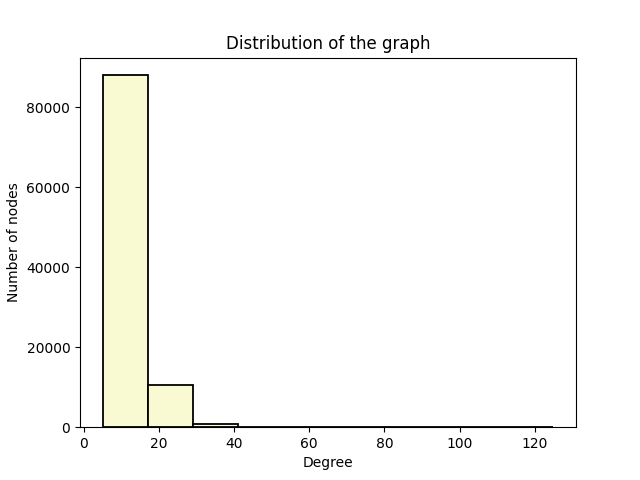
\includegraphics[width=\linewidth]{large_graphs/fe_rotor.png}  
  \caption{fe\_rotor}
  \label{fig:sub-third}
\end{subfigure}
\begin{subfigure}{.35\textwidth}
  \centering
  % include fourth image
  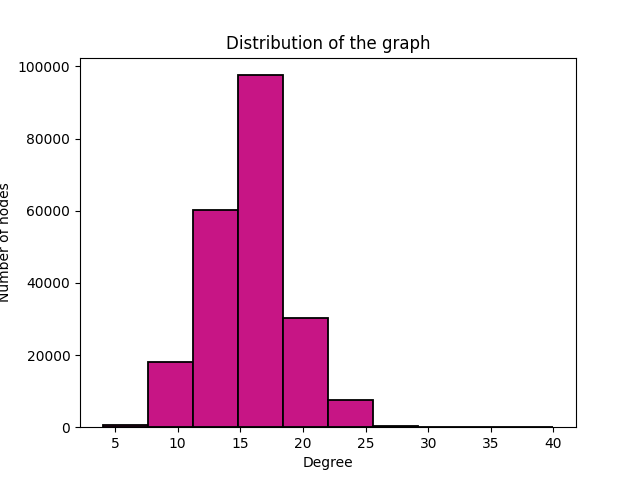
\includegraphics[width=\linewidth]{large_graphs/m14b.png}  
  \caption{m14b}
  \label{fig:sub-fourth}
\end{subfigure}
\caption{Degree histogram of large graphs. Graphs are not so dense.}
\label{fig:fig}
\end{figure}

\section{Results}

In table 

\begin{table}[h!]
\centering
\begin{tabular}{ |p{1.75cm}||cc|cc||  }
%\hline
%\multicolumn{3}{|c|}{\textbf{Results}} \\
\hline
\hline
\textbf{Graphs} & \multicolumn{2}{|c|}{\textbf{METIS}} & \multicolumn{2}{|c|}{\textbf{Modified GAP}}  \\
\hline
\hline
Name & Edge Cut & Balancedness & Edge Cut & Balancedness \\
\hline
data & 0 & 0 & 0 & 0  \\
add32 & 0 & 0 & 0 & 0  \\
bcsstk33 & 0 & 0 & 0 & 0  \\
crack & 0 & 0 & 0 & 0  \\
\hline
fe\_body & 0 & 0 & 0 & 0   \\
t60k & 0 & 0 & 0 & 0  \\
wing & 0 & 0 & 0 & 0  \\
finan512 & 0 & 0 & 0 & 0  \\
\hline
fe\_rotor & 0 & 0 & 0 & 0  \\
598a & 0 & 0 & 0 & 0  \\
m14b & 0 & 0 & 0 & 0  \\
auto & 0 & 0 & 0 & 0  \\
\hline
\end{tabular}
\caption{\label{tab:comp_graphs}Comparison of the results obtained by different algorithms in the computation graphs}
\end{table}

